\chapter{Diseño del circuito impreso} \chapterlabel{Informe/8-PCB} \label{cap:PCB}

En este capítulo se mencionan los criterios tenidos en cuenta para el diseño del circuito impreso. Además, se muestran los esquemáticos y las imágenes del PCB desarrollados para la implementación de la placa de control mediante el uso del software Altium Designer. 

Por otra parte, se describen las consideraciones y circuitos utilizados para las fuentes de alimentación del sistema.



\section{Fuentes de alimentación}

\subsection{Fuente de alimentación externa de $24\:V$}

\noindent La fuente externa se encarga de alimentar todo el circuito. Debe ser capaz de suministrar $24\:V$ y hasta $30\:A$. Para ello se puede utilizar una fuente de laboratorio o baterías.

\subsection{Fuente de alimentación interna de $12\:V$}

\noindent La fuente de $12\:V$ se encarga de alimentar al regulador de $5\:V$ y al driver del puente H. Debido a los bajos consumos de potencia y bajo costo, se utiliza una fuente lineal. Por lo tanto, se decide utilizar el integrado L78M12CDT-TR.

\subsection{Fuente de alimentación interna de $5\:V$}

La fuente de $5\:V$ se encarga de alimentar los operacionales, el sensor de efecto Hall, el inversor y el regulador de tensión de $2.5\:V$. Debido a los bajos consumos de potencia y bajo costo, se utiliza una fuente lineal. Por lo tanto, se decide utilizar el integrado L78M05CDT.

\section{Esquemáticos}

\subsection{Principal}
\begin{figure}[H]
	\centering
	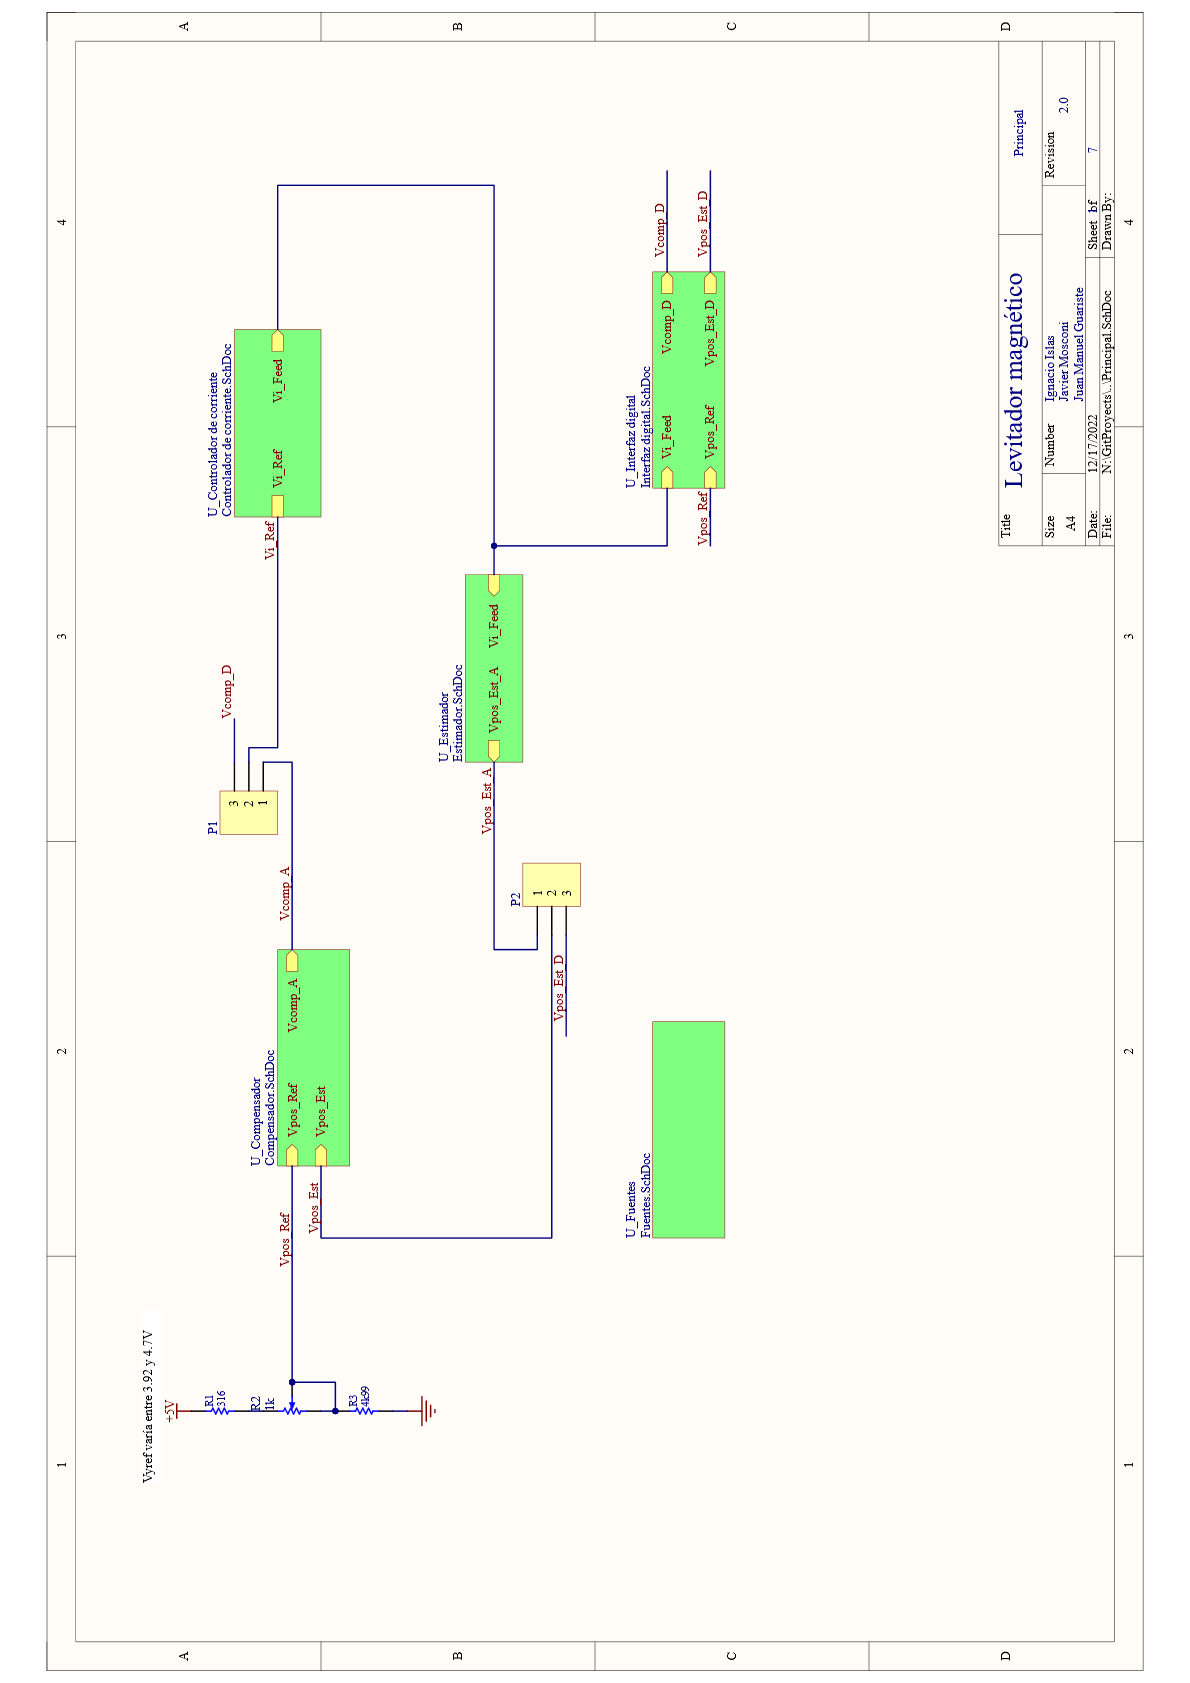
\includegraphics[scale=0.3]{main.png}
	%\caption{Diagrama en bloques de la implementación digital.}
	\label{fig:main}
\end{figure}

\subsection{Controlador de corriente}
\begin{figure}[H]
	\centering
	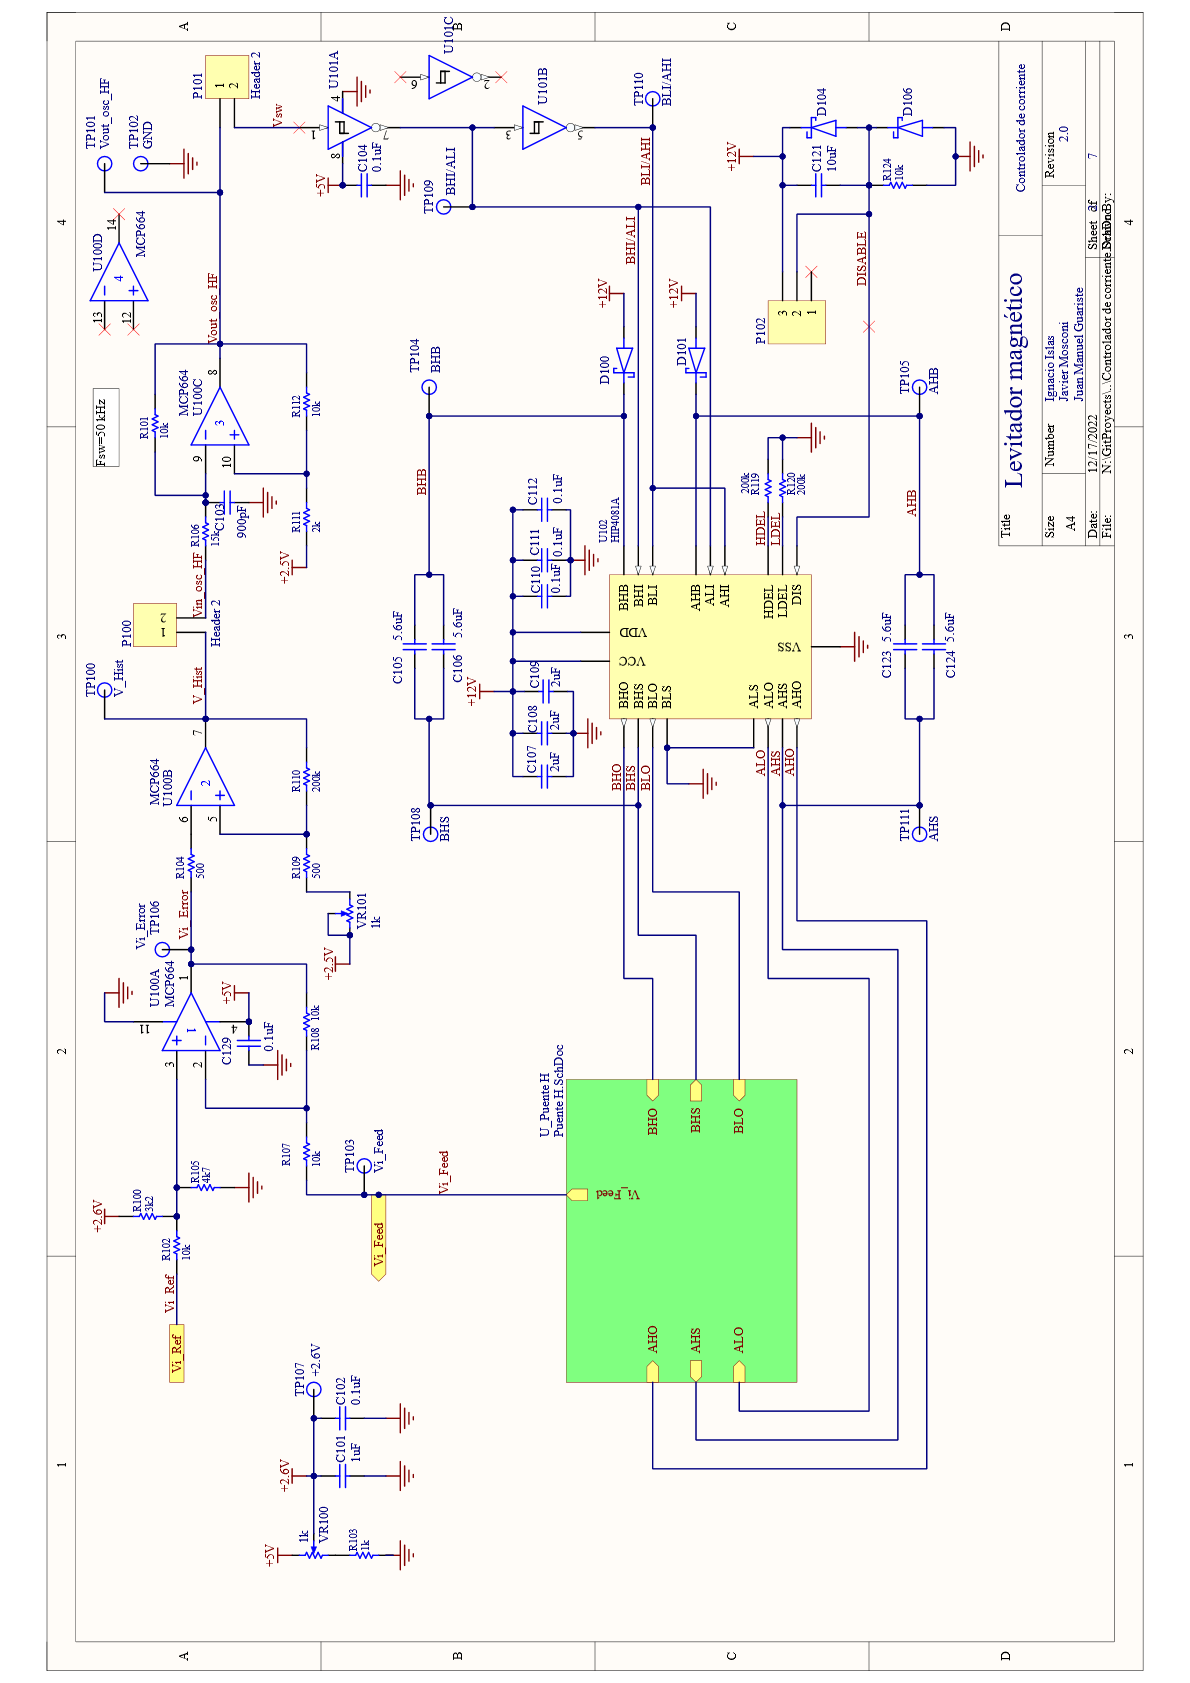
\includegraphics[scale=0.32]{contCorrEsq.png}
	%\caption{Diagrama en bloques de la implementación digital.}
	\label{fig:contCorrEsq}
\end{figure}

\subsection{Puente H}
\begin{figure}[H]
	\centering
	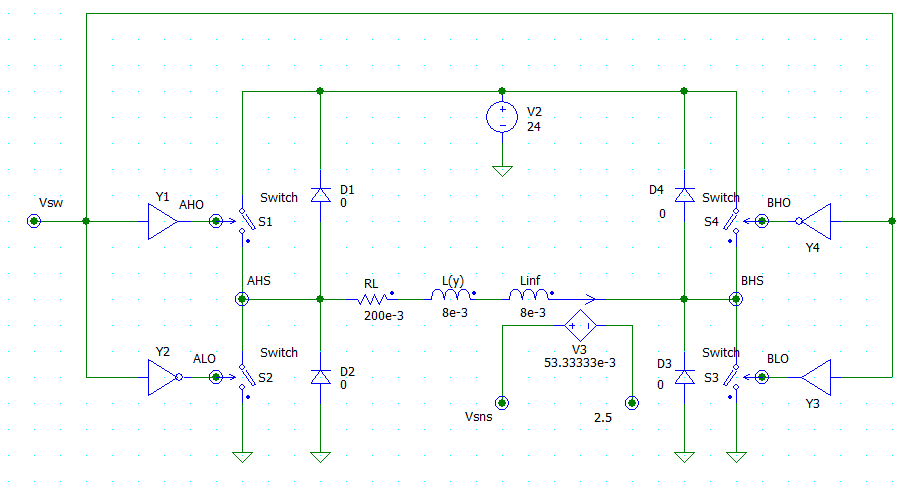
\includegraphics[scale=0.32]{PuenteH.png}
	%\caption{Diagrama en bloques de la implementación digital.}
	\label{fig:PuenteH}
\end{figure}

\subsection{Compensador analógico}
\begin{figure}[H]
	\centering
	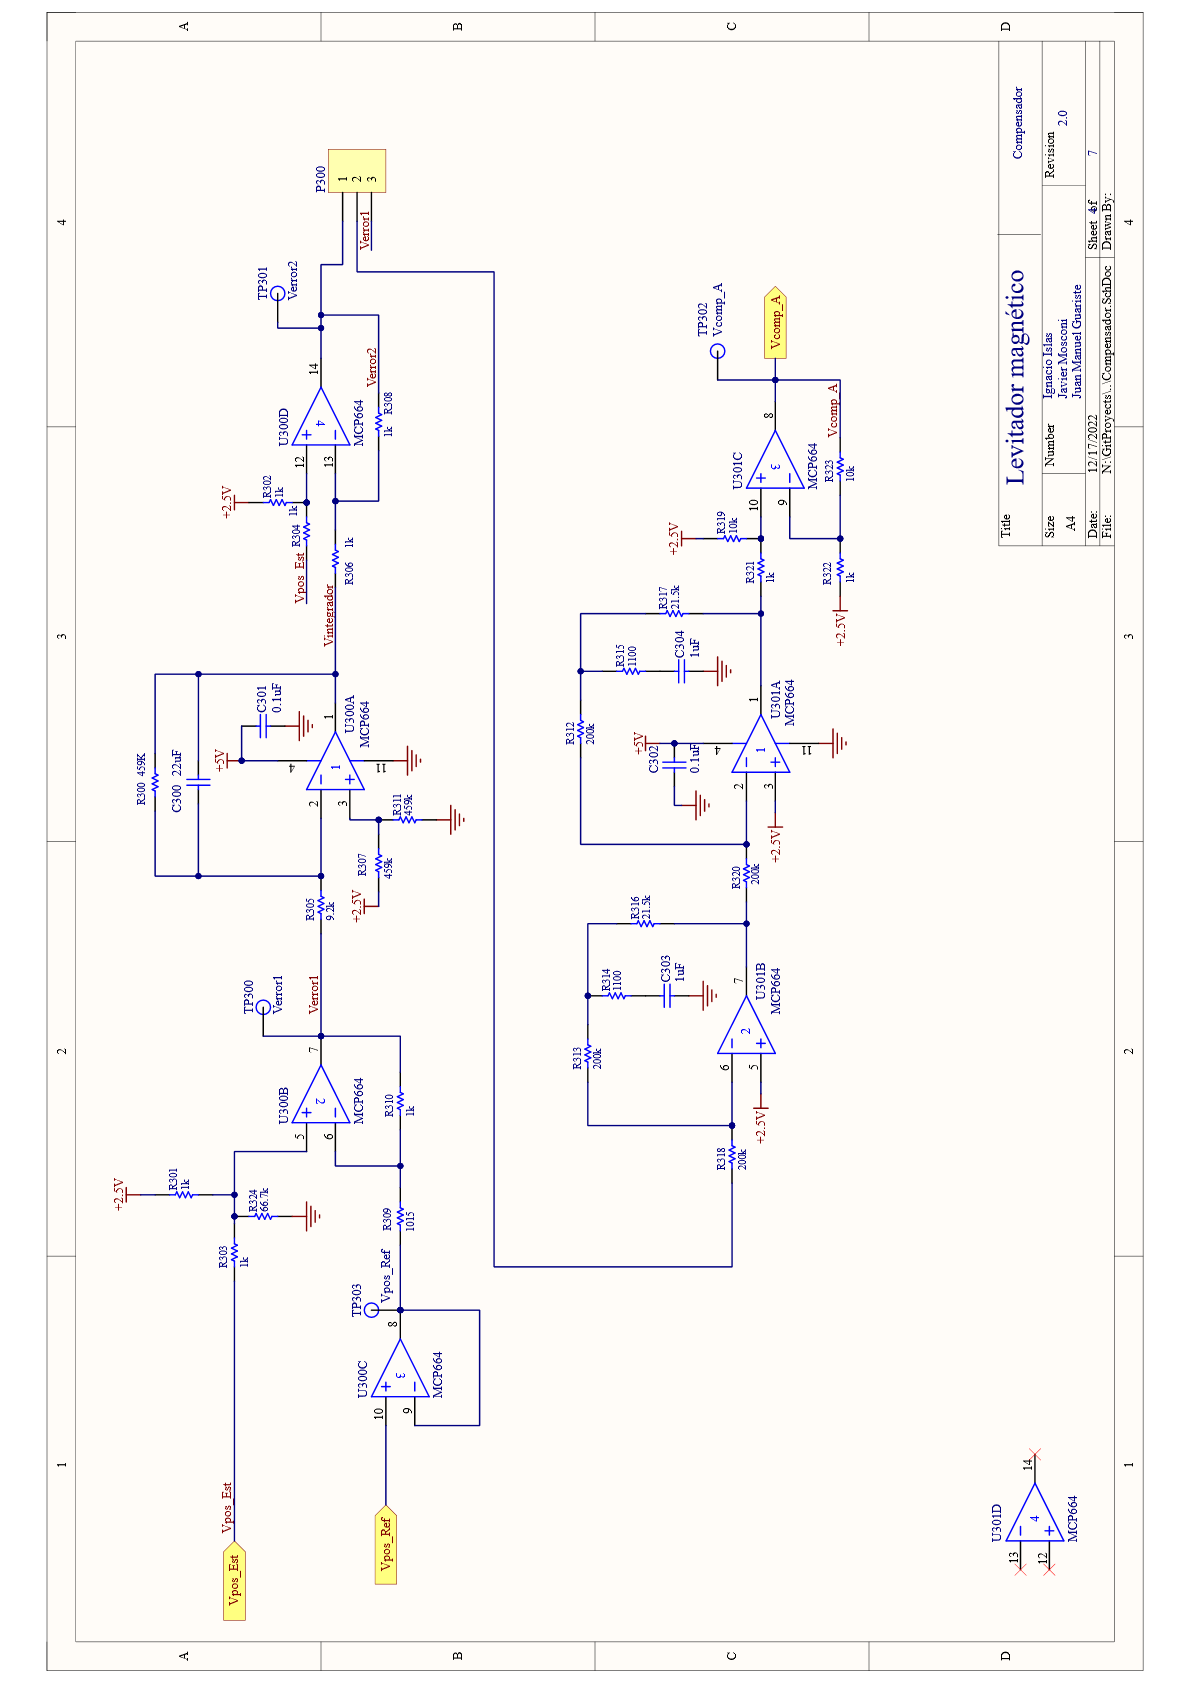
\includegraphics[scale=0.32]{CompAnalog.png}
	%\caption{Diagrama en bloques de la implementación digital.}
	\label{fig:CompAnalog}
\end{figure}

\subsection{Estimador analógico}
\begin{figure}[H]
	\centering
	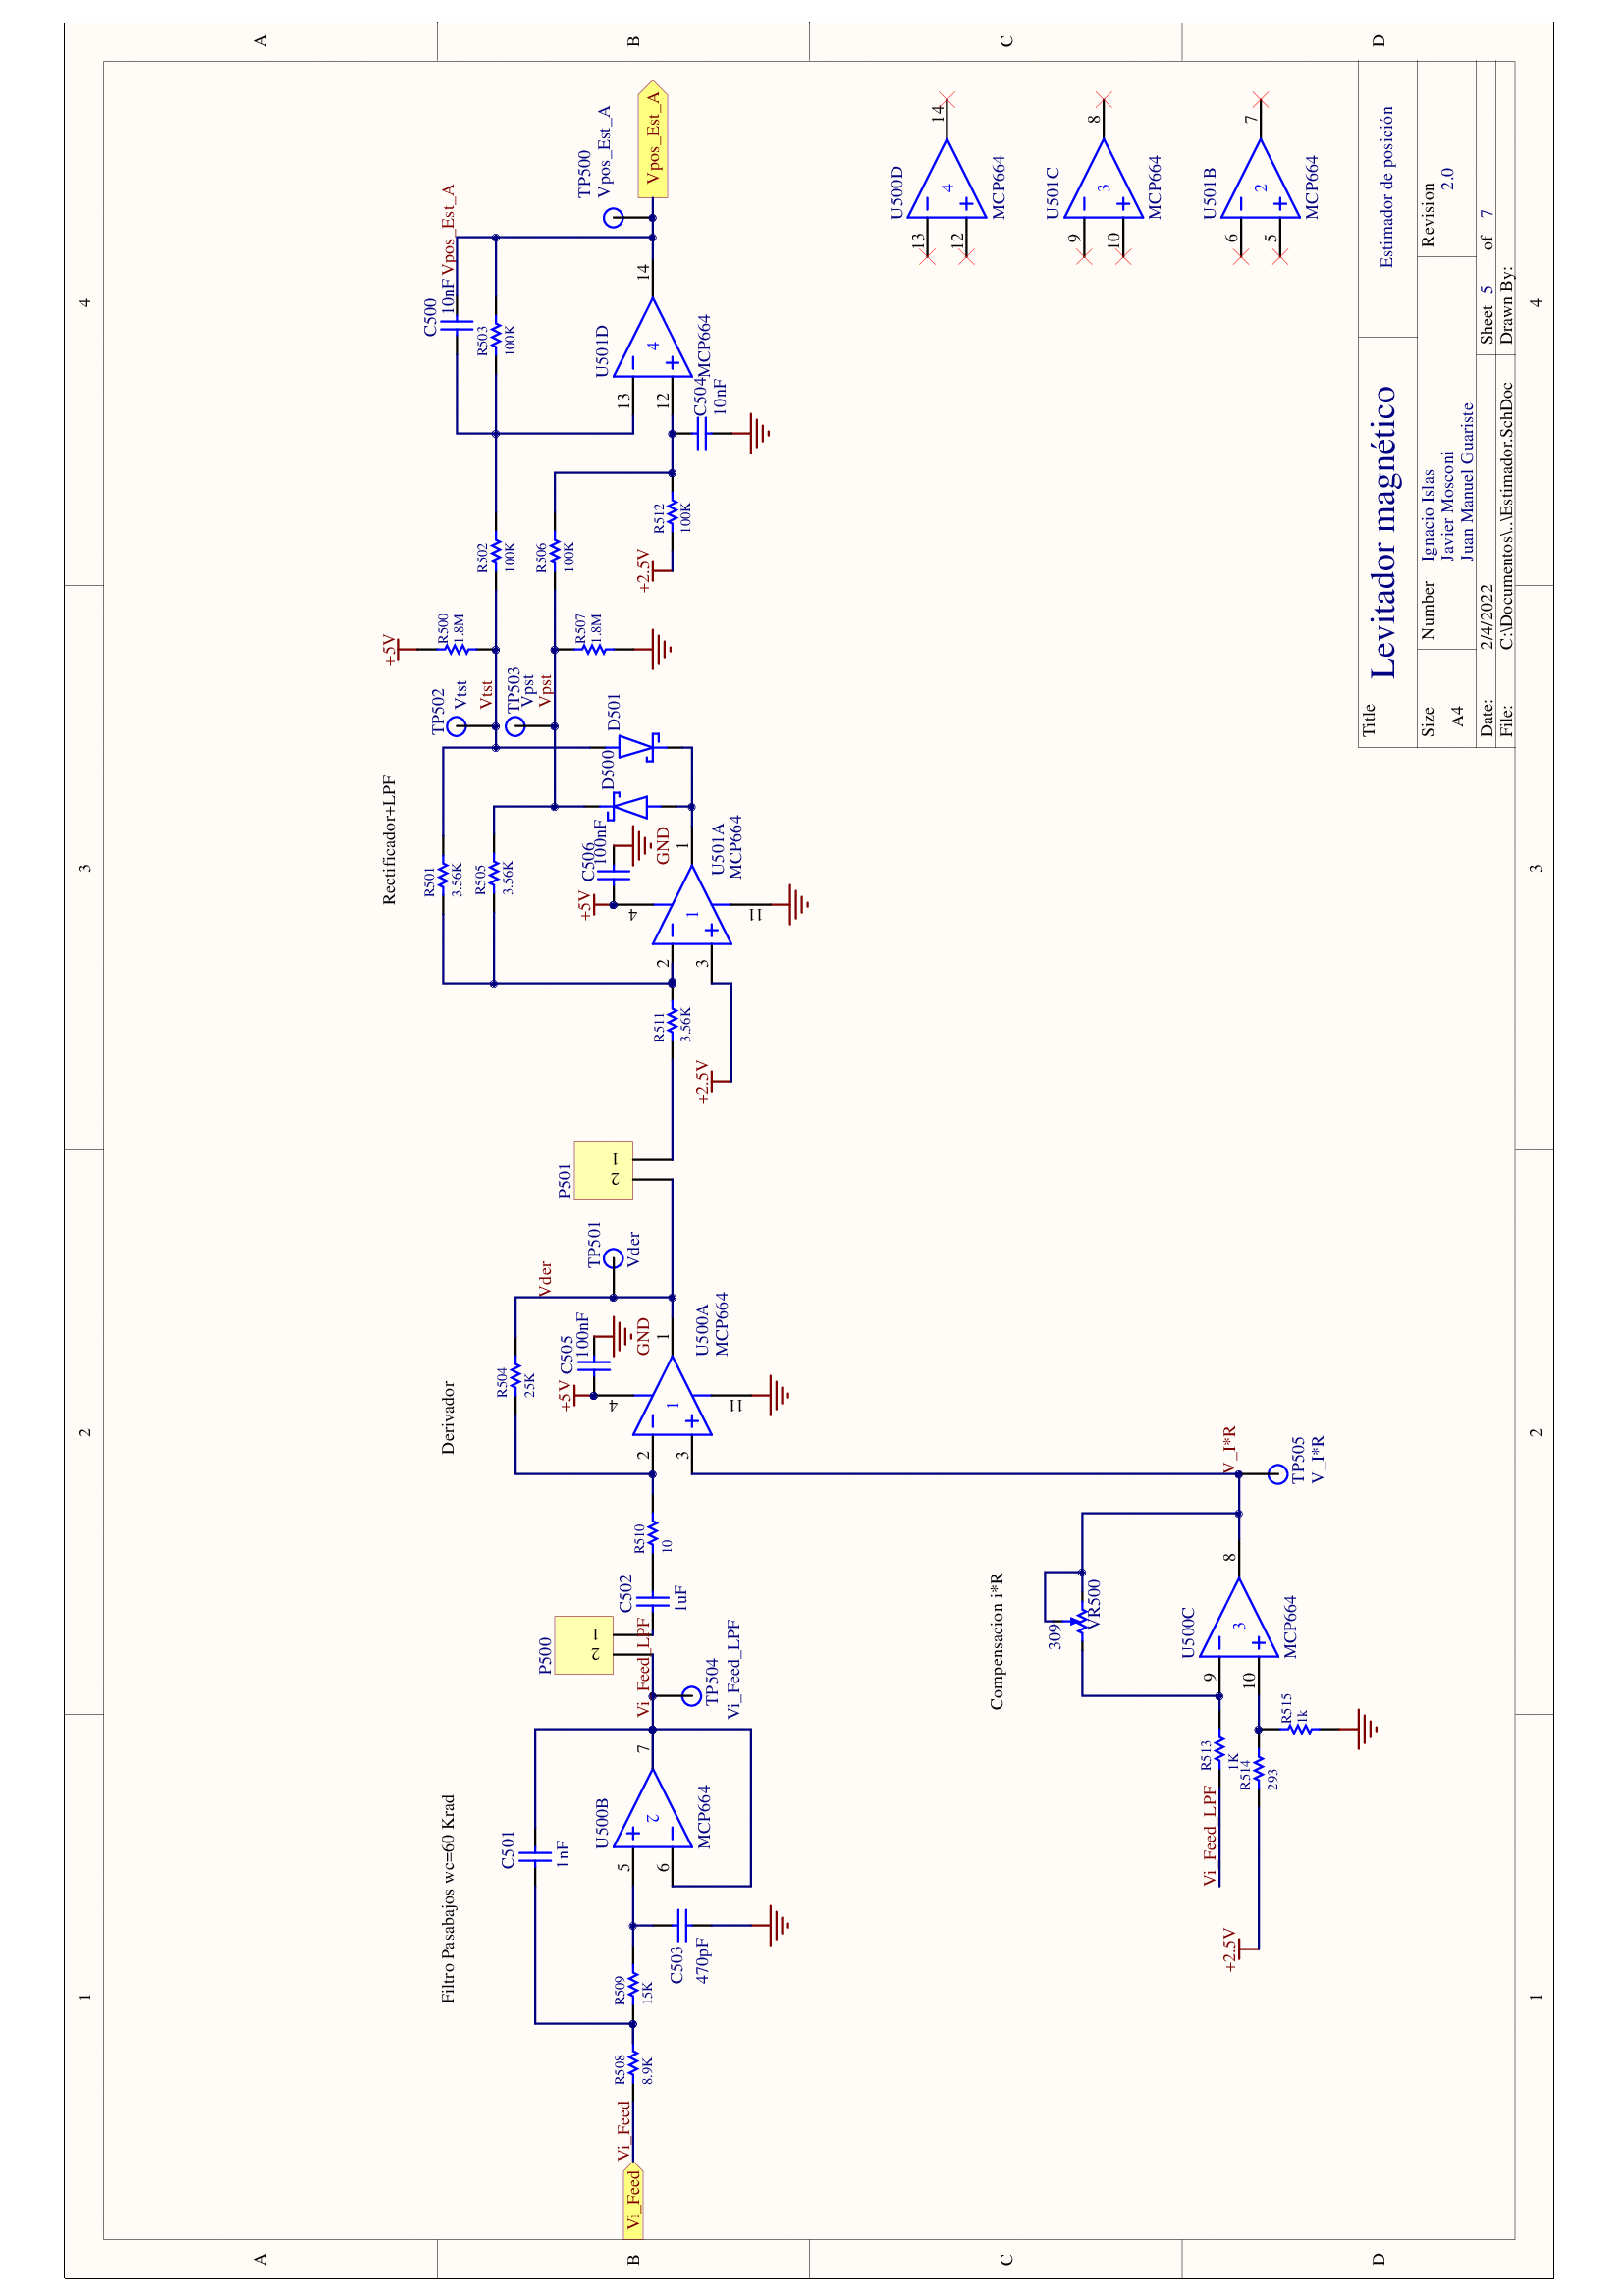
\includegraphics[scale=0.32]{EstimAnalog.png}
	%\caption{Diagrama en bloques de la implementación digital.}
	\label{fig:EstimAnalog}
\end{figure}

\subsection{Interfaz con microcontrolador}
\begin{figure}[H]
	\centering
	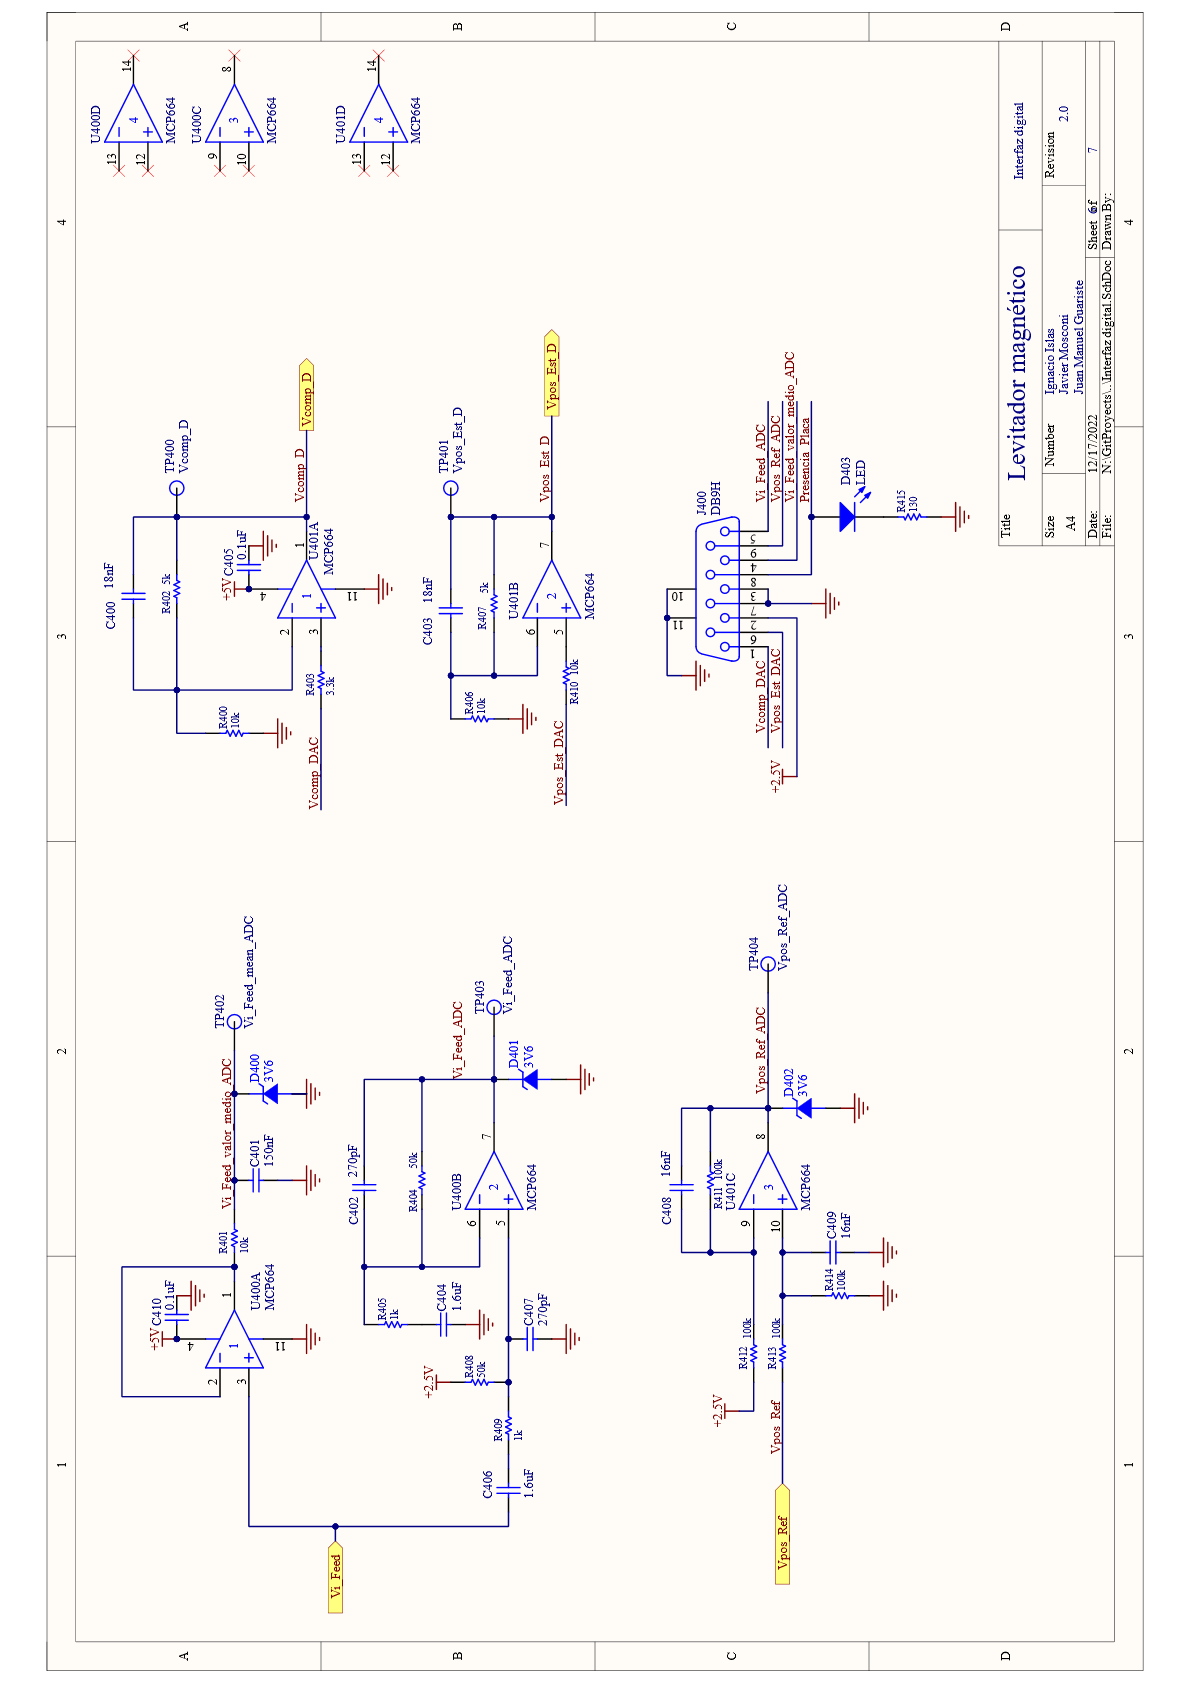
\includegraphics[scale=0.32]{InterfazMic.png}
	%\caption{Diagrama en bloques de la implementación digital.}
	\label{fig:InterfazMic}
\end{figure}

\subsection{Fuentes de alimentación}
\begin{figure}[H]
	\centering
	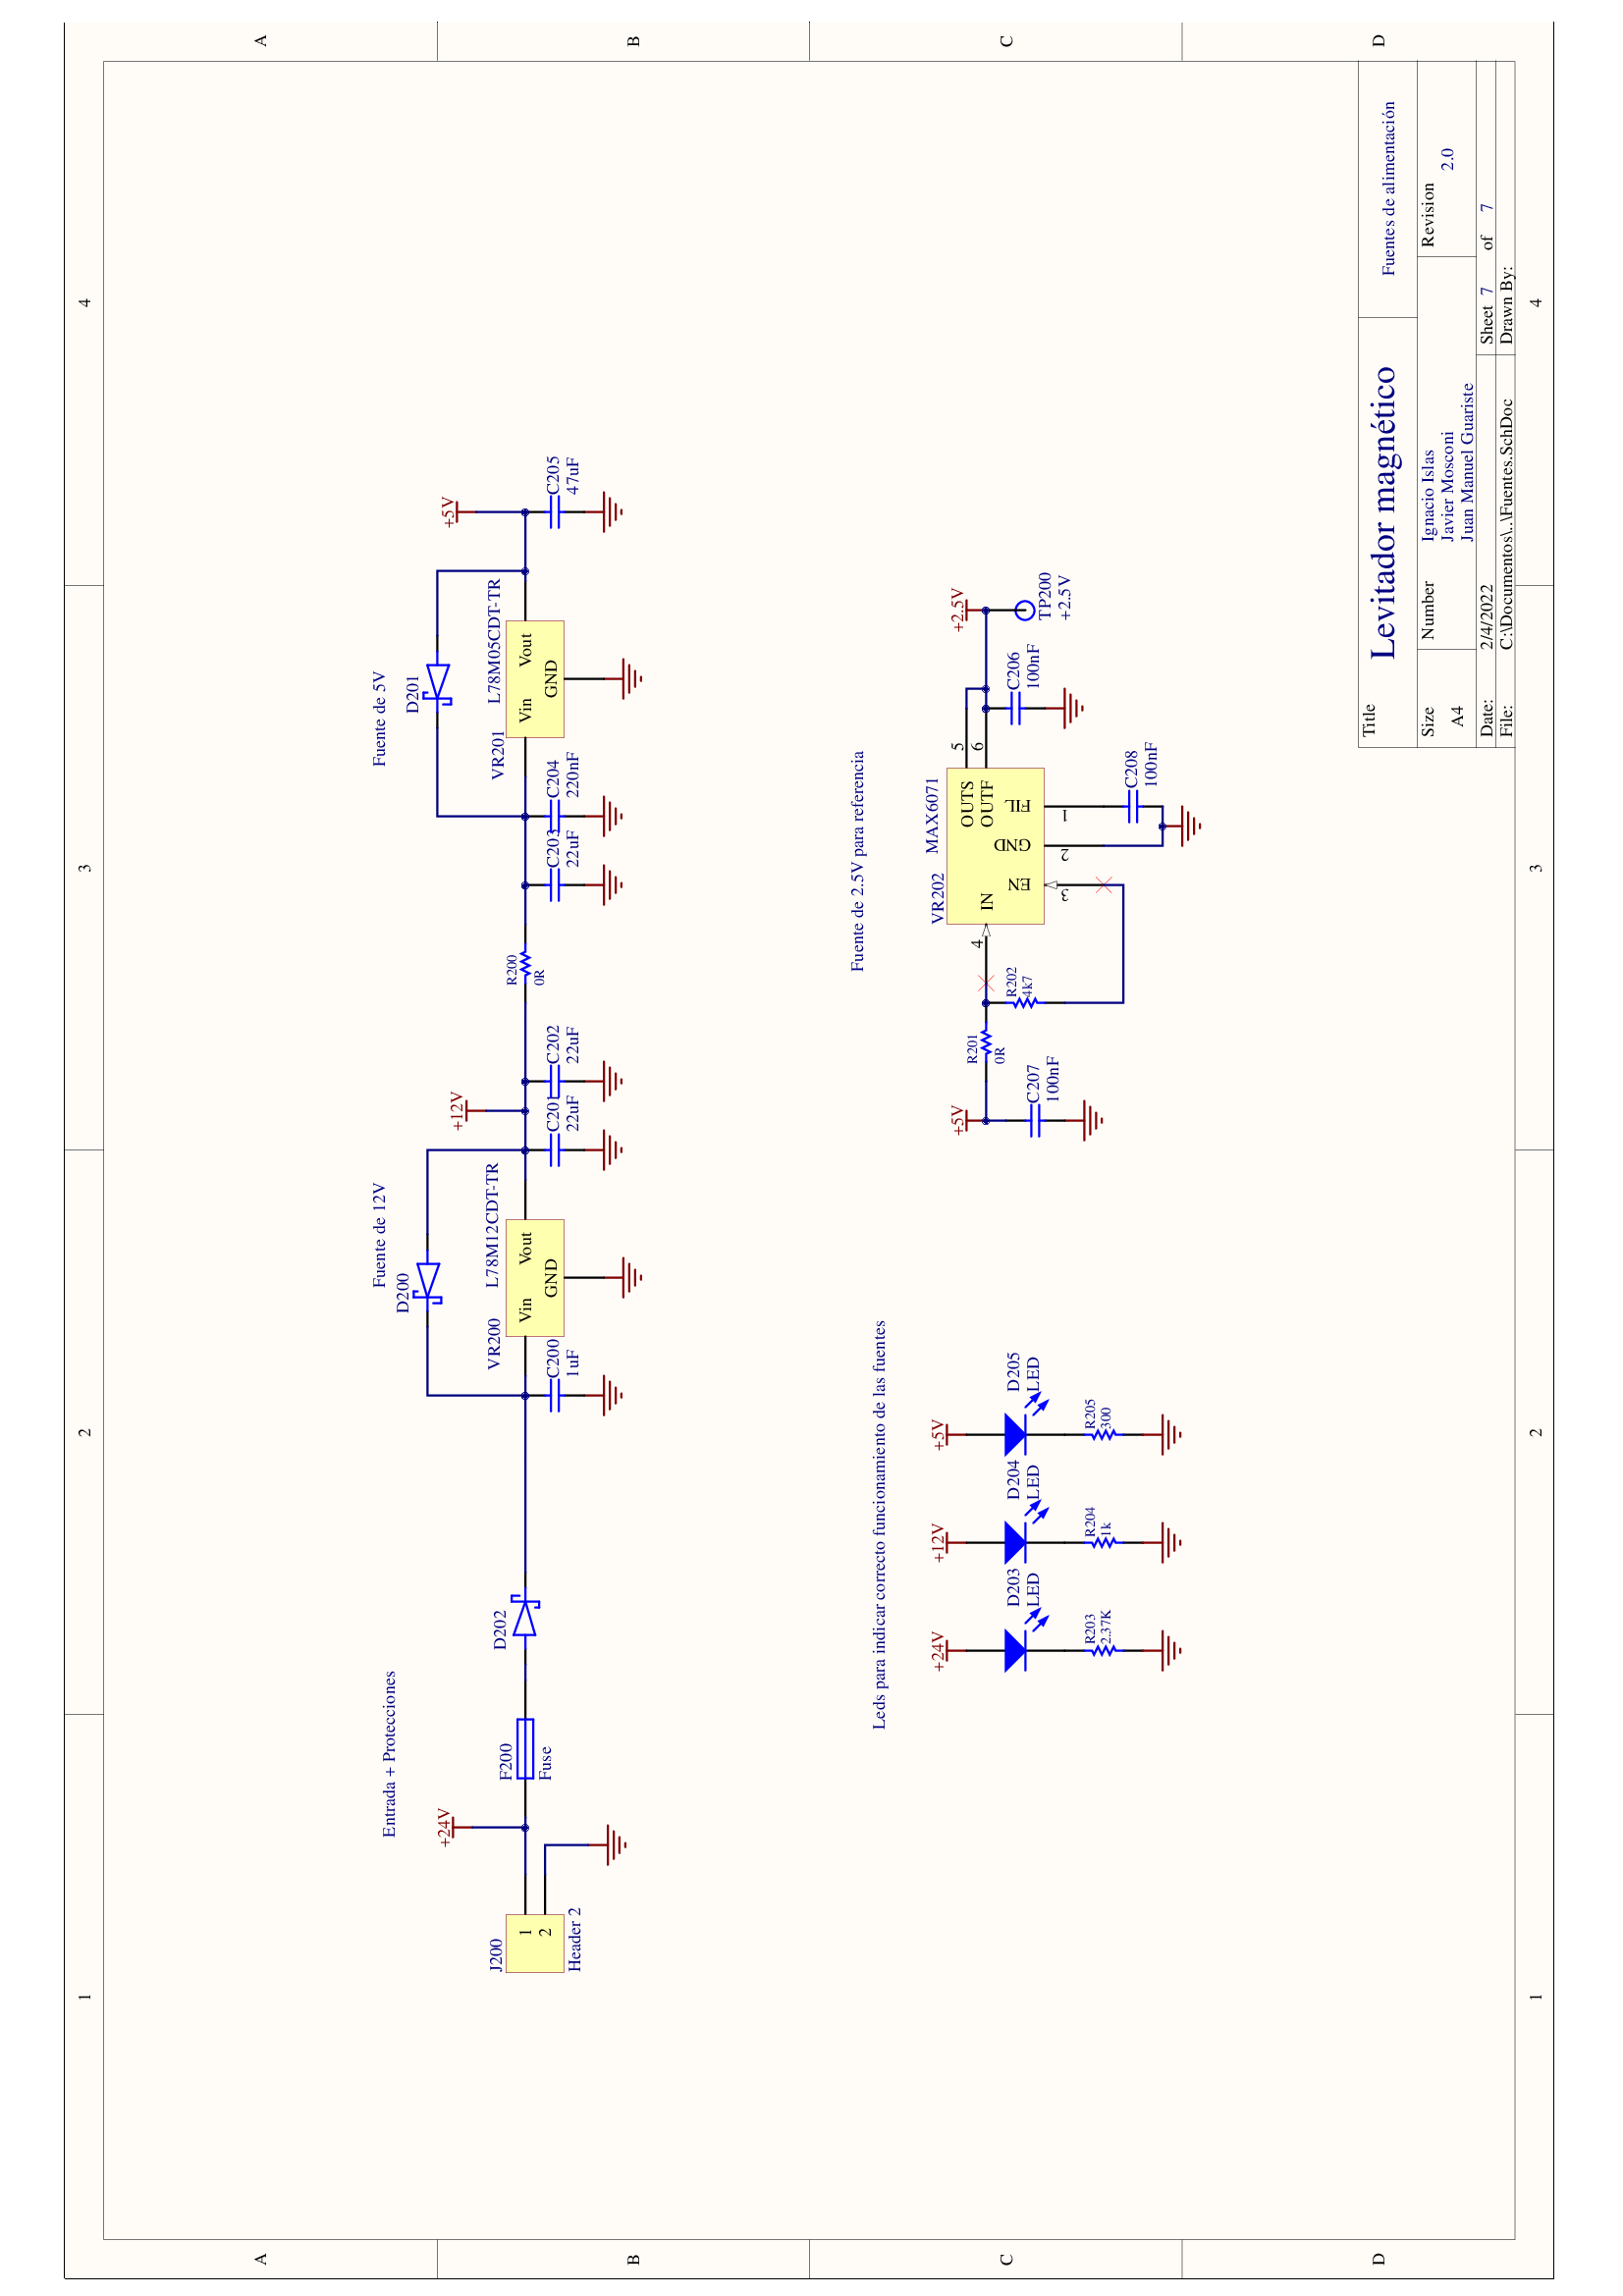
\includegraphics[scale=0.3]{FuentesAliment.png}
	%\caption{Diagrama en bloques de la implementación digital.}
	\label{fig:FuentesAliment}
\end{figure}

\section{PCB}
\subsection{Consideraciones para el diseño del PCB}
Para el diseño del PCB se tuvieron en cuenta los siguientes aspectos:

\begin{itemize}
	\item Se utilizó un plano de masa para la etapa de potencia y otro para el resto del circuito. Se intentó reducir al mínimo las conexiones entre ambos planos con el objetivo de disminuir el ruido inducido por la etapa de potencia en el resto del circuito.
	\item Se mantuvo separada la etapa de potencia con las de pequeña señal.
	\item Se intentó reducir al mínimo la longitud de las pistas de las señales críticas como la tensión de salida del sensor de efecto Hall.
	\item Se utilizaron pistas gruesas y polígonos para la etapa de potencia que deben soportar la circulación de corrientes elevadas.
	\item Se quitó la capa ``Top Solder'' en la etapa de potencia correspondiente al puente H para mejorar la disipación.
	\item Se pusieron vías en toda la placa para ayudar a la disipación de potencia y a la disminución del ruido. 
	\item Se ``acostaron'' los MOSFET sobre la placa para ayudar a su disipación de potencia.
	\item Se realizó el diseño en una placa de 2 capas para reducir el costo de fabricación.
	\item Para optimizar el tamaño de la placa, se rutearon las pistas de manera organizada. Para ello, se intentó que las pistas verticales se realicen en la capa superior mientras que las horizontales, en la inferior.
	\item El proyecto se dividió en 7 esquemáticos. Cada uno de ellos se asocia a una etapa en específico. Por ejemplo uno de ellos está destinado a la etapa de compensación analógica, otro al estimador analógico, etc. A su vez, los componentes de cada esquemático tiene asociado un rango de valores determinados para los ``designators''. Es decir, todos los componentes con ``designators'' entre 0 y 99 pertenecen al primer esquemático, los de 100 a 199 al segundo, y así sucesivamente.  De esta forma, con solo ver el ``designators'' en el PCB es posible determinar, fácilmente, a qué etapa pertenece.  
	\item Se siguieron las reglas de diseño estándar de PCBWay.
	
\end{itemize}



 






\subsection{Modelo 2D}
\subsubsection{Vista superior}
\begin{figure}[H]
	\centering
	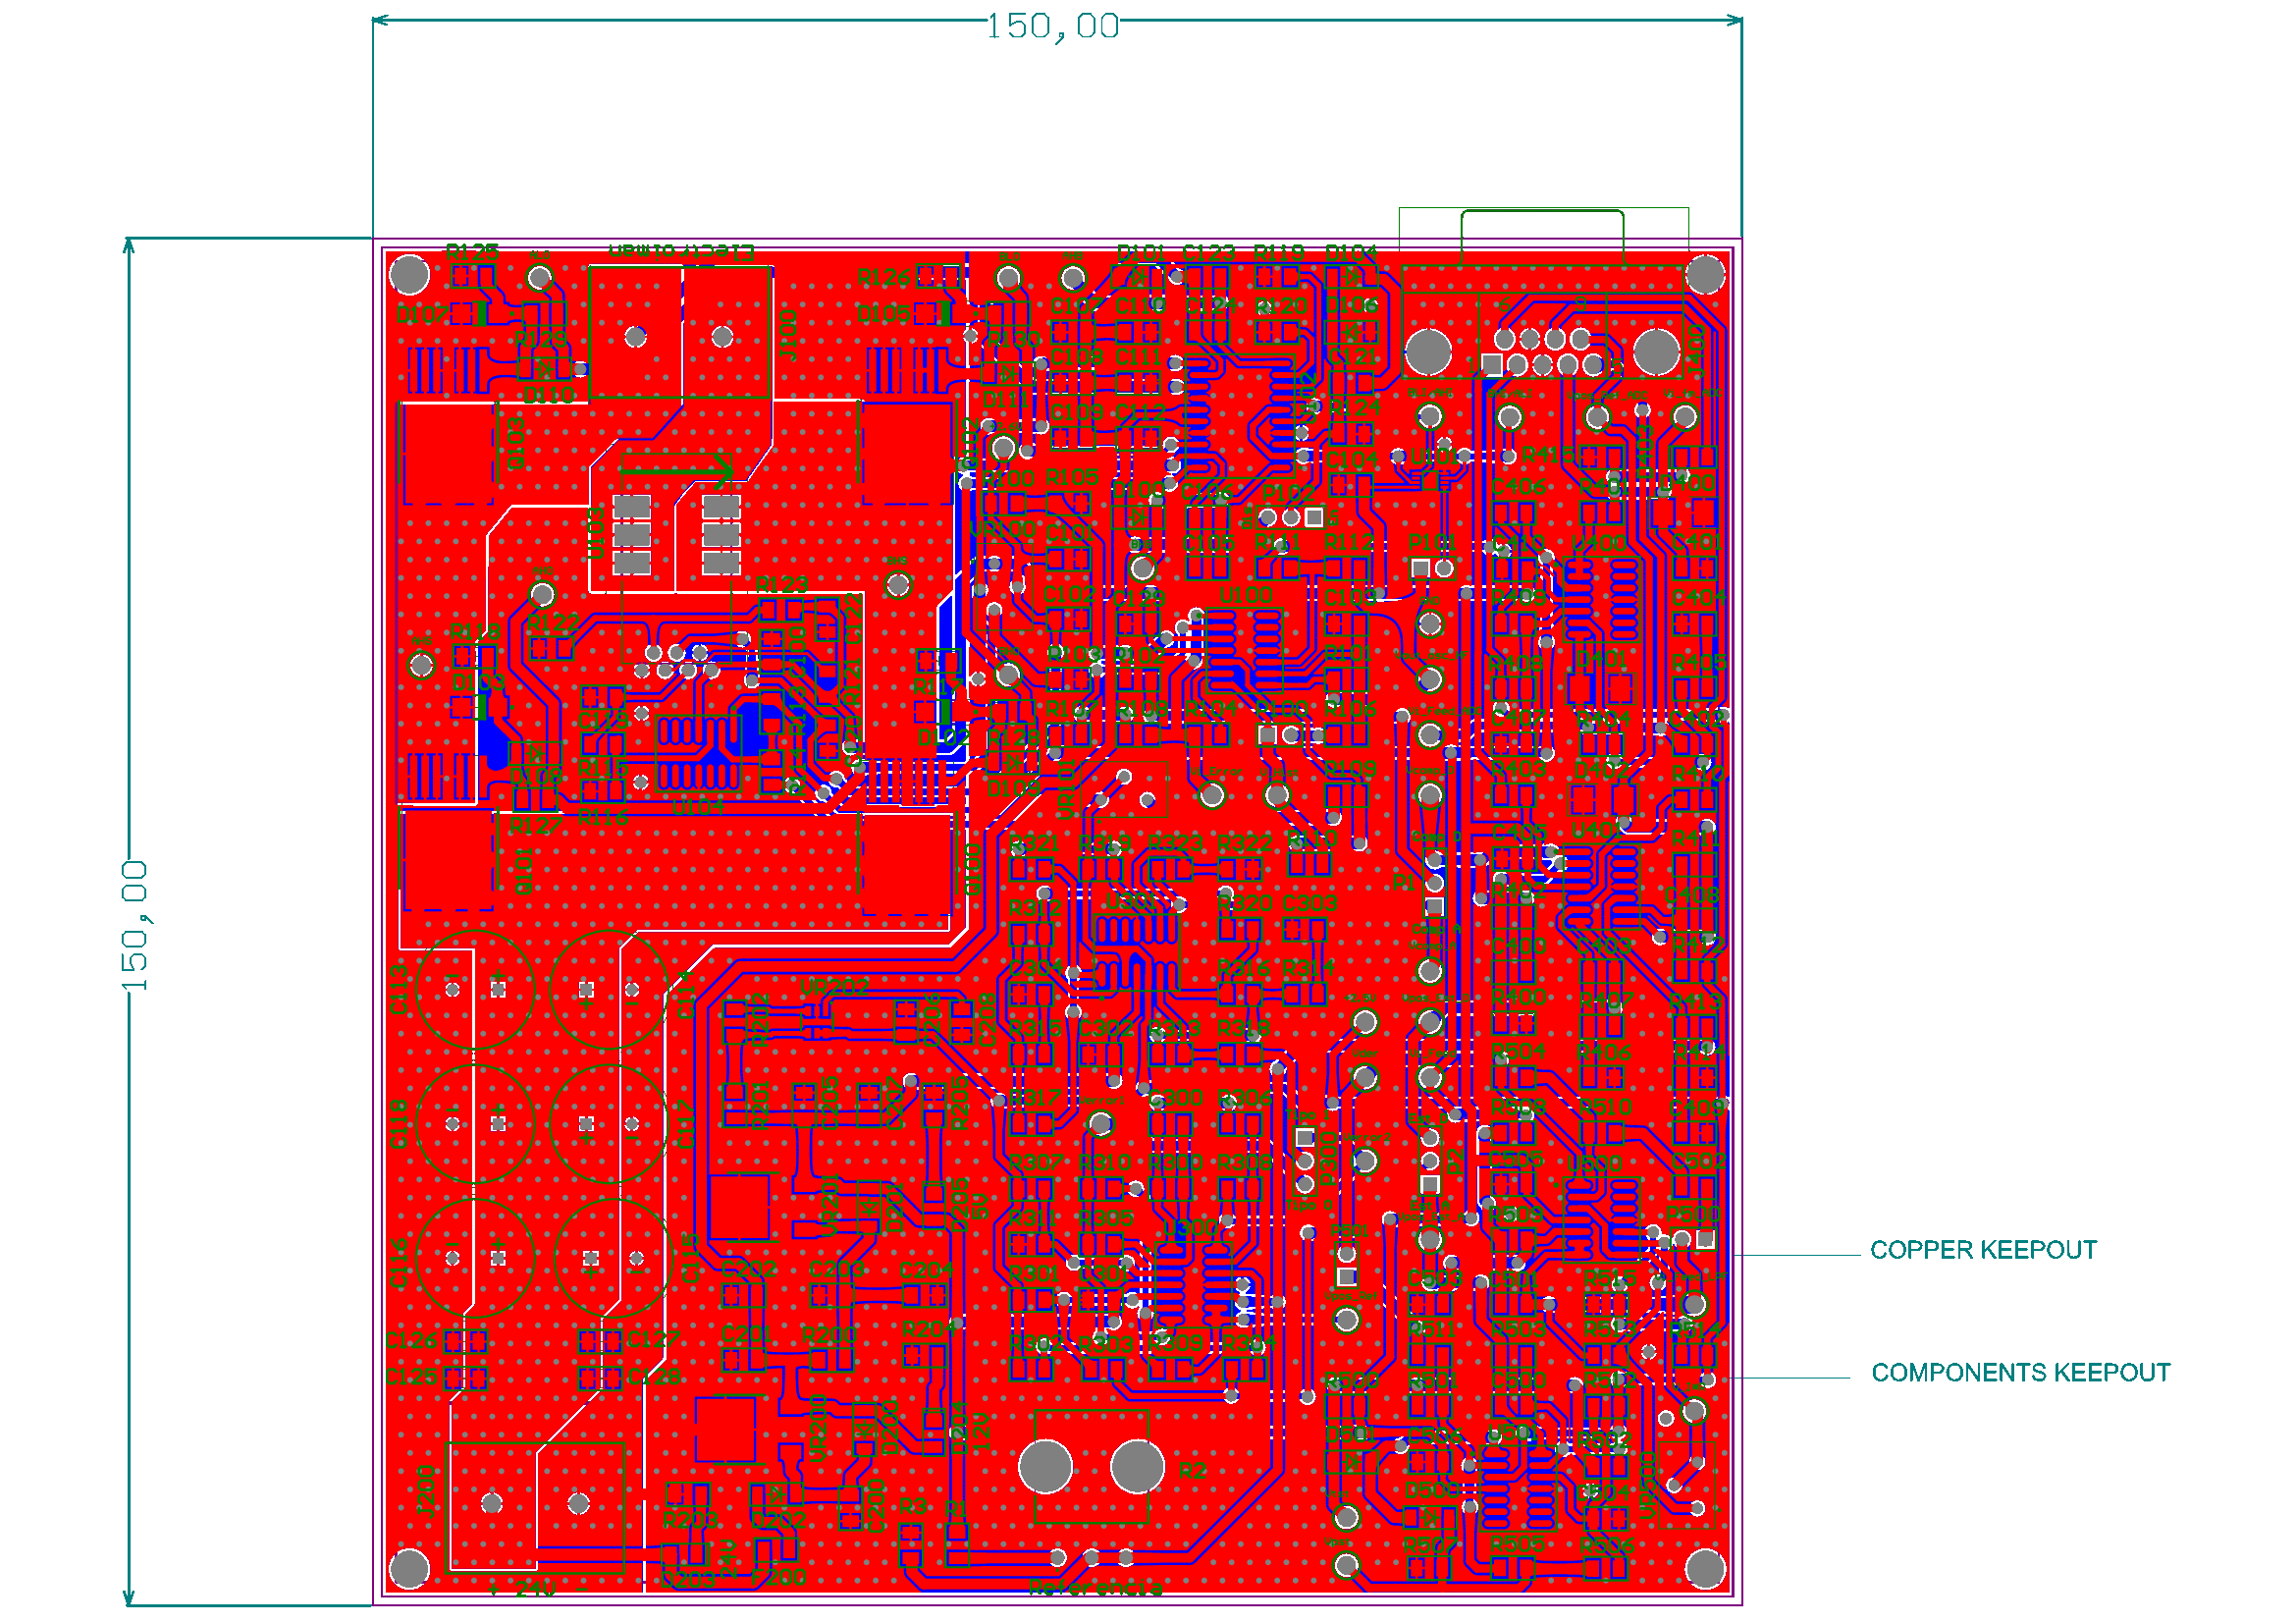
\includegraphics[scale=0.2]{VistSup.png}
	%\caption{Diagrama en bloques de la implementación digital.}
	\label{fig:VistSup}
\end{figure}

\subsubsection{Vista inferior}
\begin{figure}[H]
	\centering
	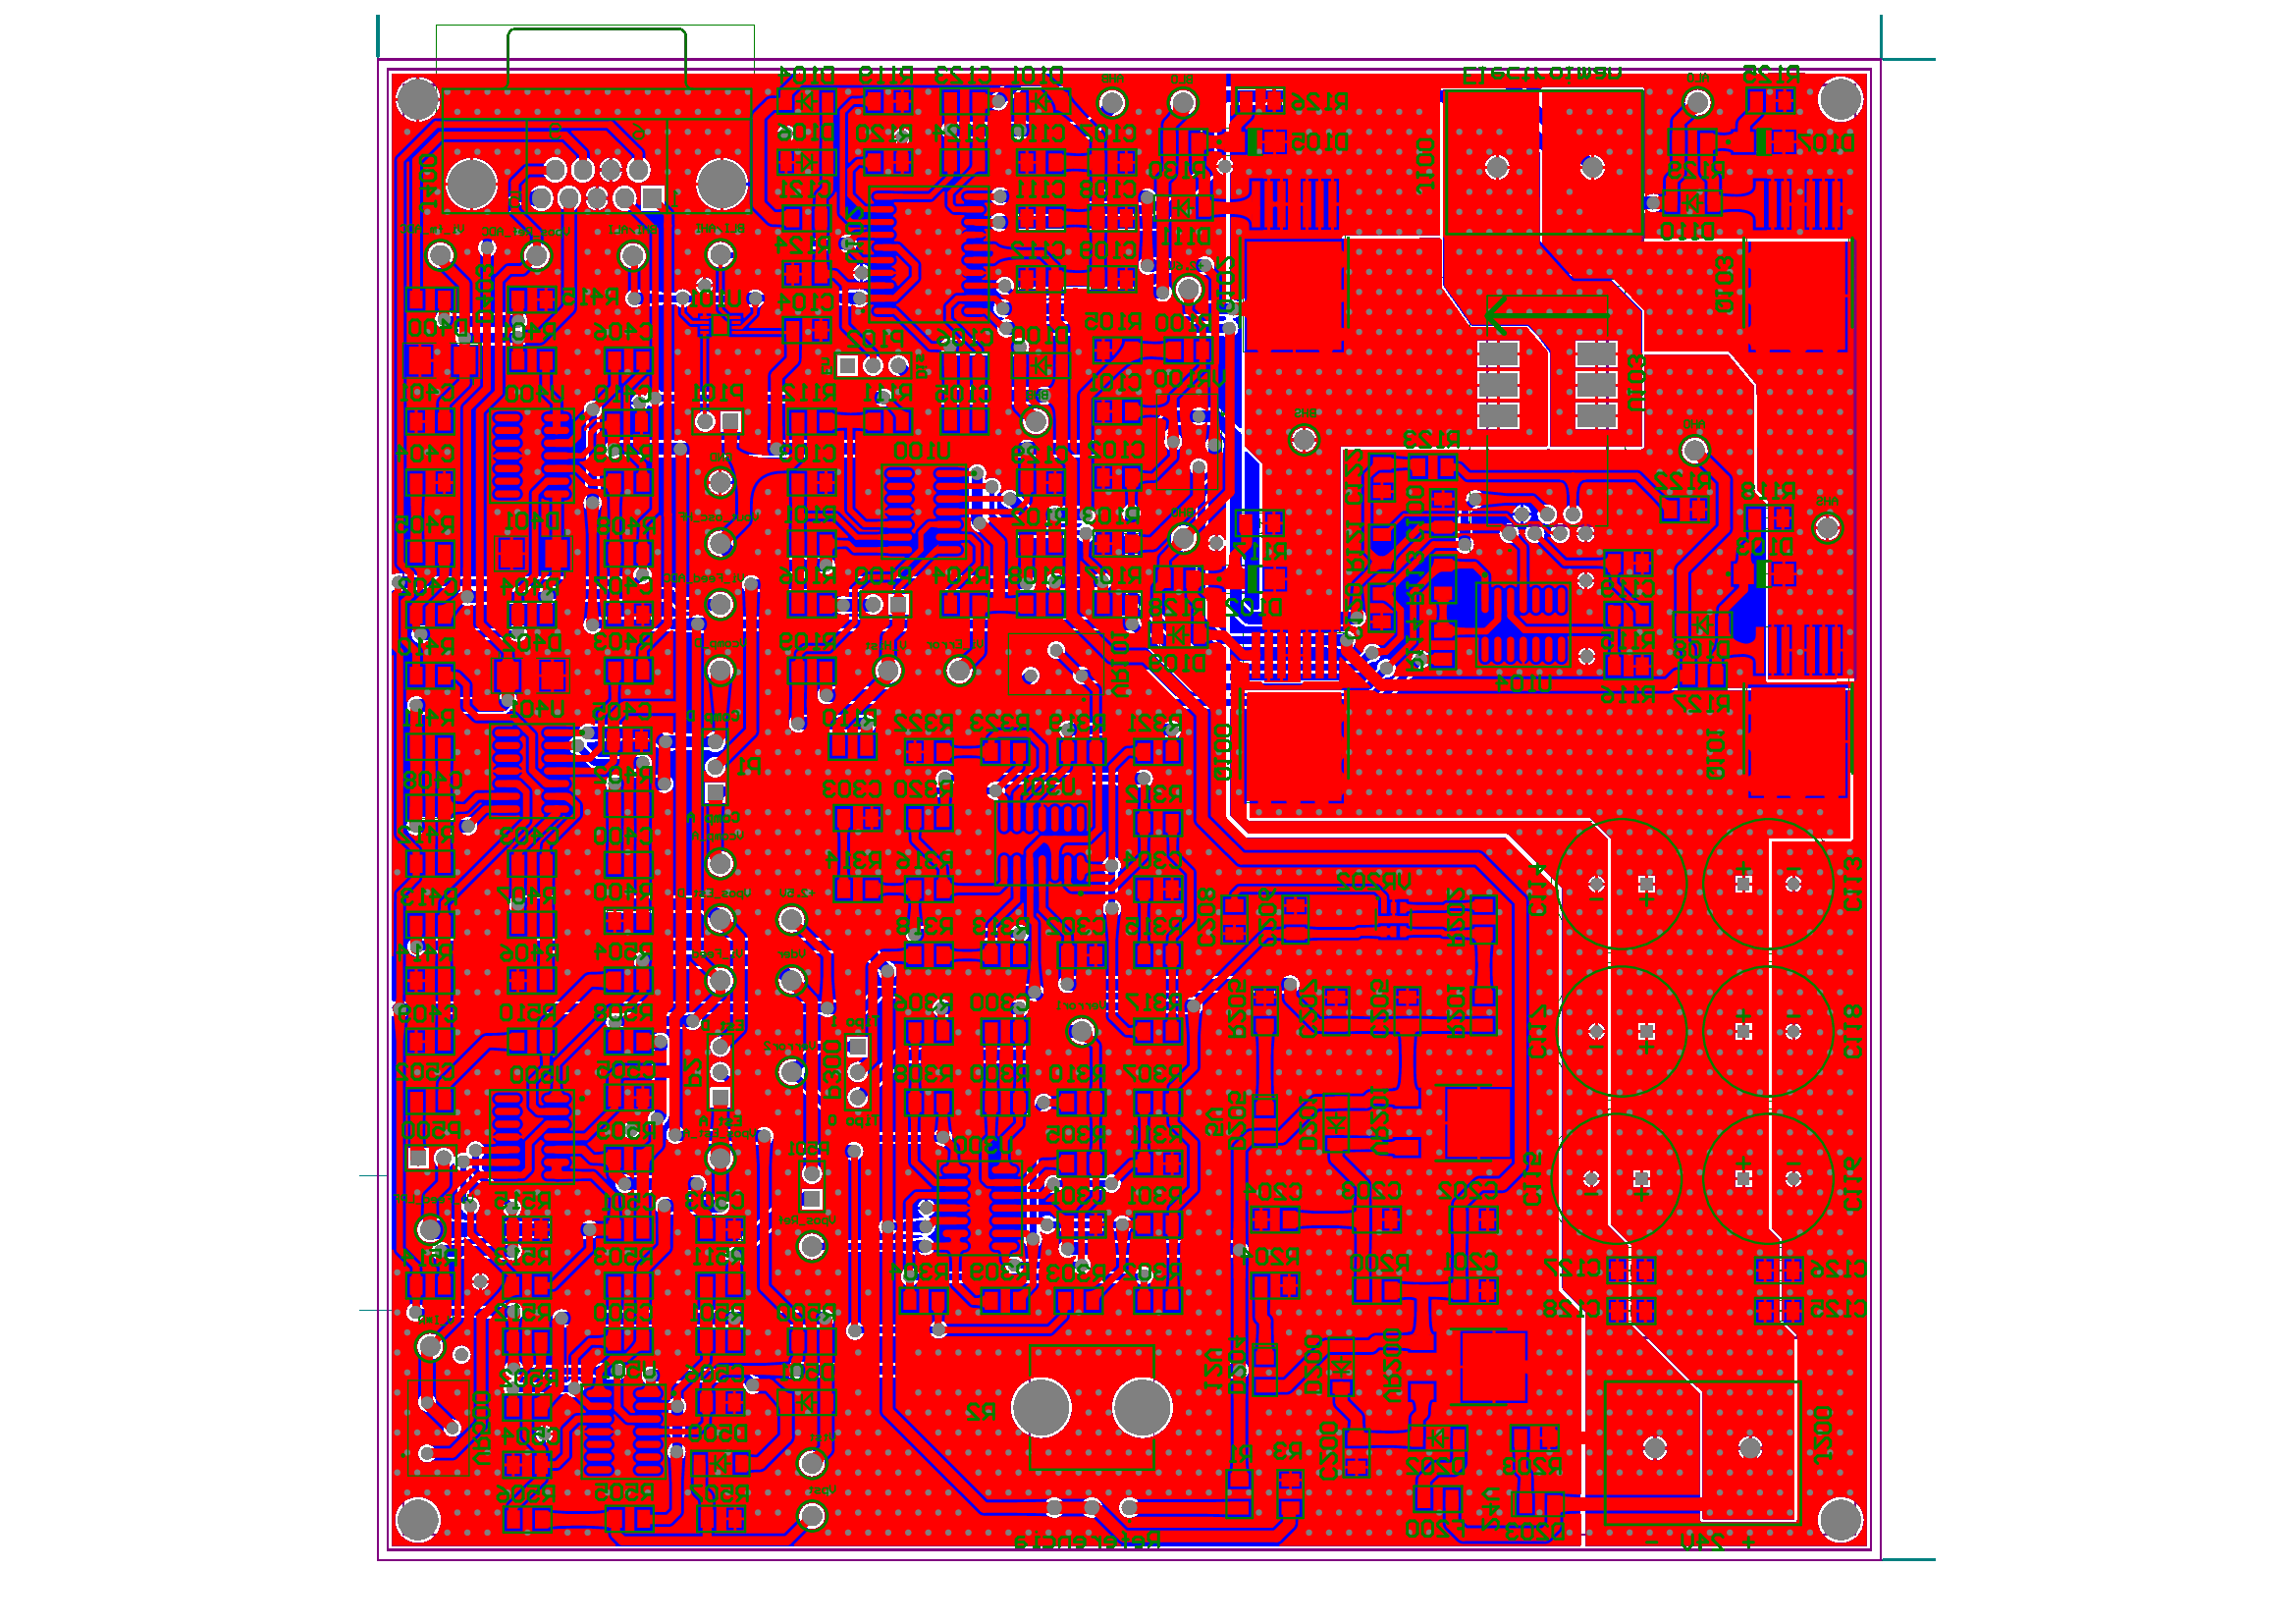
\includegraphics[scale=0.2]{VistInf.png}
	%\caption{Diagrama en bloques de la implementación digital.}
	\label{fig:VistInf}
\end{figure}

\subsection{Modelo 3D}
\subsubsection{Vista superior}
\begin{figure}[H]
	\centering
	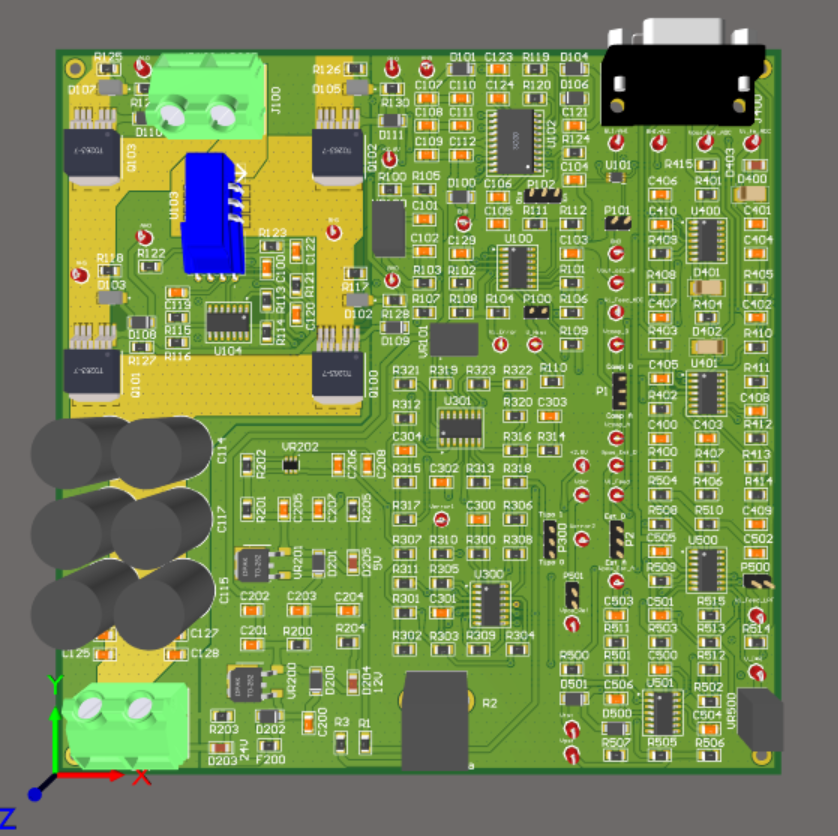
\includegraphics[scale=0.3]{VistSup3D.png}
	%\caption{Diagrama en bloques de la implementación digital.}
	\label{fig:VistSup3D}
\end{figure}

\subsubsection{Vista inferior}
\begin{figure}[H]
	\centering
	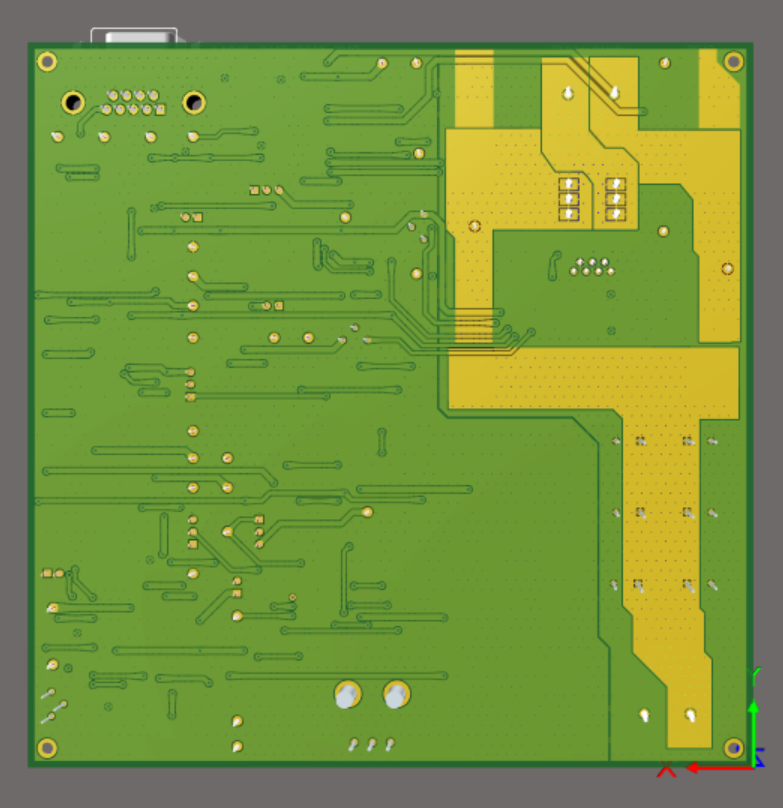
\includegraphics[scale=0.3]{VistInf3D.png}
	%\caption{Diagrama en bloques de la implementación digital.}
	\label{fig:VistInf3D}
\end{figure}

